\section{Simulation Procedure} \label{sec:sim_procedure}

Now that a flight certification maneuver has been chosen, a method to run a current aircraft design thorough the maneuver-of-interest needs to be be developed.
The aircraft design is represented using probabilistic multi-fidelity aerodynamics and controls databases as shown in \ref{sec:gtt_dbs}.
The uncertainty in the data that informs the databases, manifests itself in slight variations in the samples of the databases.
Each sample aerodynamic database has information about the forces and moments on an aircraft at various points in the flight envelope.
The controls database samples contain information about the moments induced on the aircraft due to various control surface deflections. 
These samples are run through flight simulation software that can integrate the force and moment information, combine it with the effects of control inputs, and perform a time-accurate maneuver that is defined in the simulation software. 

This part of the work leans heavily on the expertise of the The Boeing Company in flight simulation and control law mixing.
Due to proprietary and patent restrictions, exact implementation of the flight simulation code is unavailable but enough information is provided to outline the simulations' overarching methodology and workflow.

Figure \ref{fig:cfr147d_inputs} represents the steps required to simulate the airworthiness test. 
The first step in the simulation process is to convert the maneuver of interest, in this case the \textit{Lateral Control: Roll Capability \S 25.147(d)} maneuver, into a trajectory for the aircraft to follow. 
This maneuver is mostly defined by roll angle of the aircraft and is shown in Figure \ref{subfig:roll_angle}.
There are other parameters included in the trajectory definition, for example constant altitude to ensure a steady level turn, but the roll angle is of primary concern and is focused on here. 
The aircraft starts with steady level flight, rolls to an angle $\psi = +30^\circ$, and then completes the roll maneuver from $\psi = +30^\circ$ to $=-30^\circ$ in 11 seconds, as required by the certification maneuver. 

The required trajectory and 

\begin{figure}
    \centering
    \begin{subfigure}[Flight simulation trajectory definition for the roll angle of the aircraft. Derived from the air-worthiness test.] {
        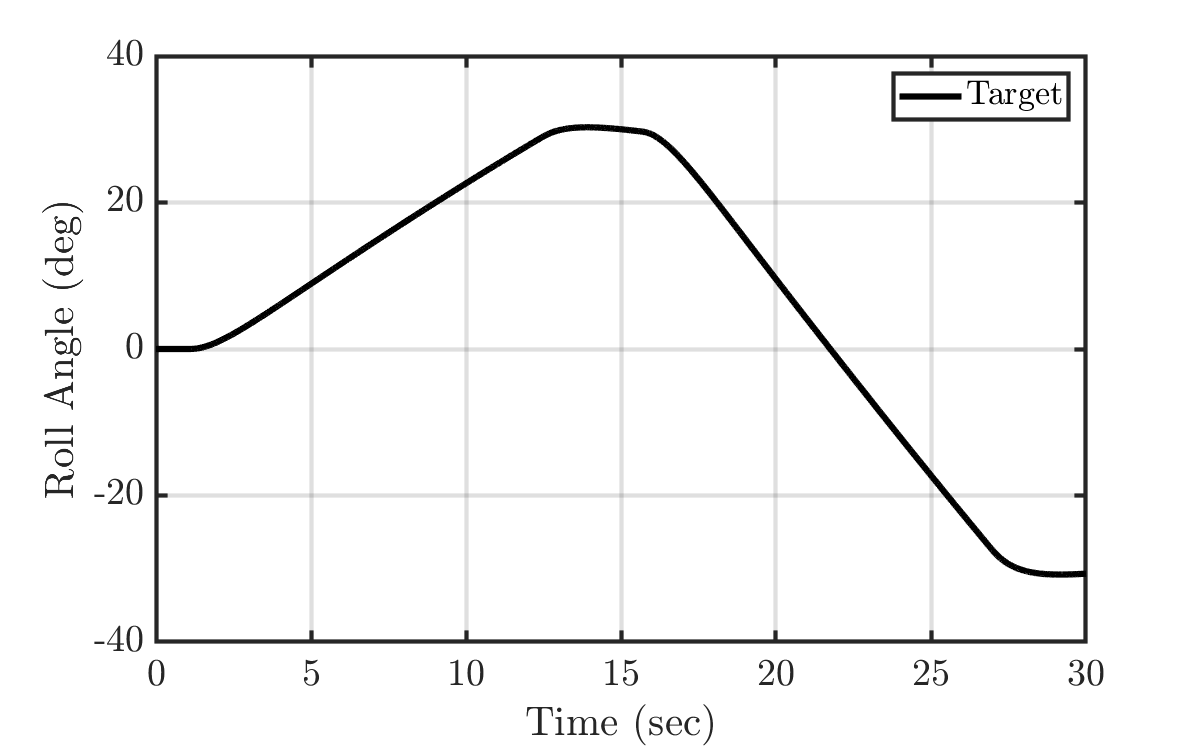
\includegraphics[trim=0 0 0 0, clip, width=.55\textwidth]{suthesis/images/cfr147d_roll_angle.png}
        \label{subfig:roll_angle}
    }
    \end{subfigure}
    \hfill
    \begin{subfigure}[Roll acceleration that would be required for the aircraft to follow the roll angle trajectory]{
        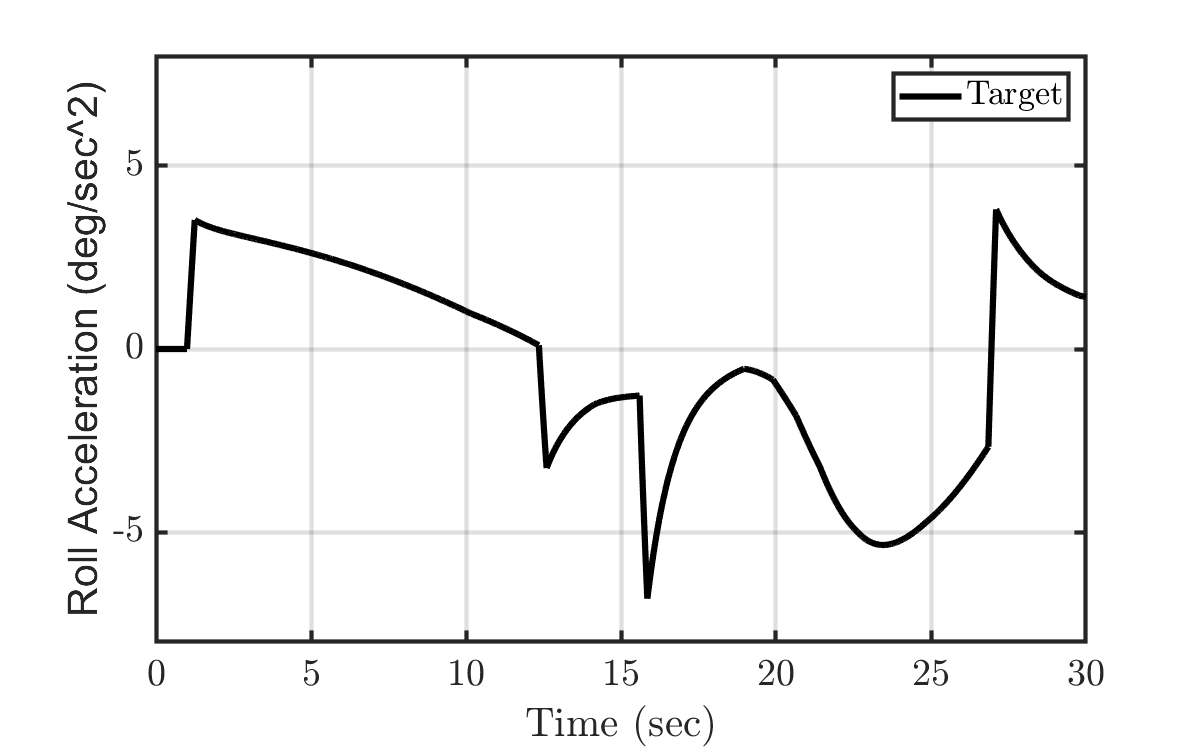
\includegraphics[trim=0 0 0 0, clip, width=.55\textwidth]{suthesis/images/cfr147d_roll_acc.png} 
        \label{subfig:roll_acc}
    } 
    \end{subfigure}
    \hfill
    \begin{subfigure}[Left and right aileron deflections commanded to create the requisite roll accelerations]{
        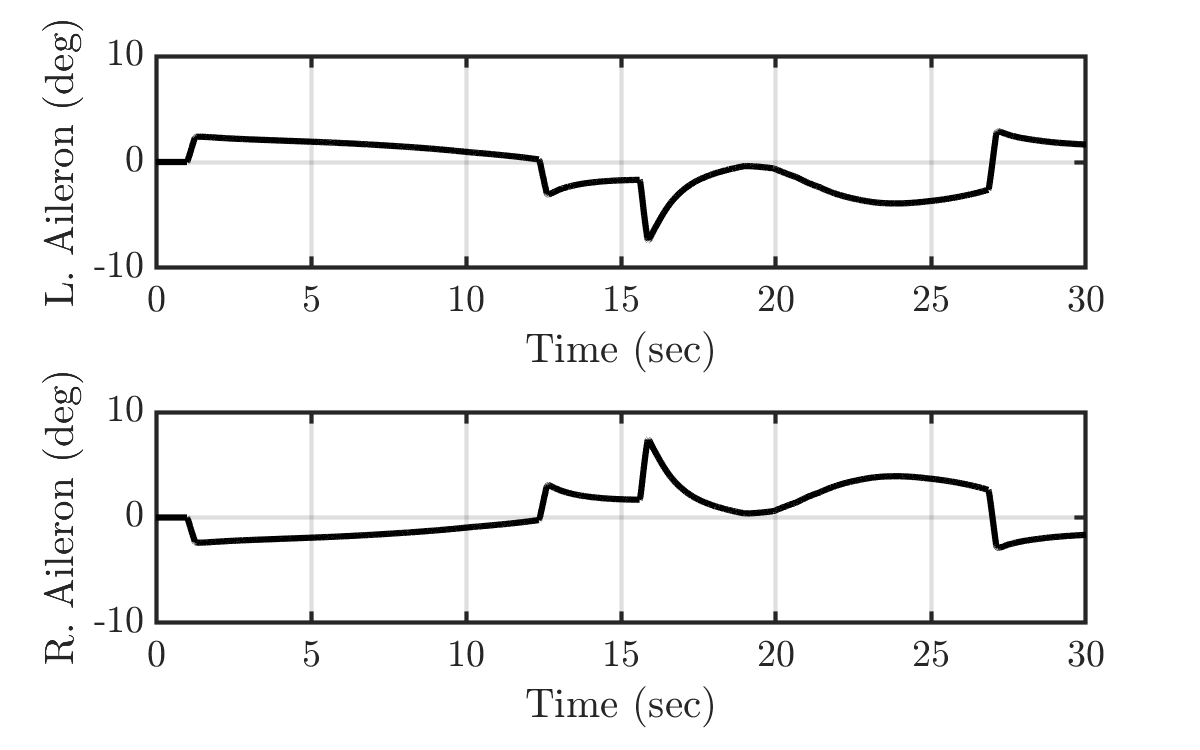
\includegraphics[trim=0 0 0 0, clip, width=.55\textwidth]{suthesis/images/cfr147d_ail_defl.png} 
        \label{subfig:ail_defl}
    } 
    \end{subfigure}
    \caption{Steps required to convert the air-worthiness test into a the required inputs for the flight simulation of the maneuver. \label{fig:cfr147d_inputs}}
\end{figure}